\subsection{Диффузионные нейронные сети}
Диффузионным нейронным сетям удалось оказать заметное влияние на сферу обработки картинок и видеорядов. Диффузионные нейронные сети являются подкатегорией глубоких генеративных моделей. Они состоят из этапов прямой и обратной диффузий и генерируют новые данные, аналогичные тем, на которых они обучались. В отличие от традиционных генеративных моделей, таких как GAN и вариационные автокодировщики (\texttt{VAE}), диффузионные модели реализуют процесс поэтапного преобразования шума в осмысленные данные, что обеспечивает высокое качество синтезируемых изображений и стабильность обучения \cite{diffusion_intro}.

Подход диффузионных нейронных сетей обусловлен неравновесной термодинамикой: модели плавно накладывают шум на объект из тренировочной выборки, а затем обучаются обращать процесс диффузии \cite{diffusion_thermo}. Целью этого процесса является получение осмысленных изображений, имеющих сходство с исходным набором данных. В отличие от \texttt{VAE}, где латентное пространство ограничено и требуется оптимизация вариационной нижней оценки, диффузионные модели используют фиксированную процедуру зашумления и обладают латентным пространством высокой размерности, что способствует более гибкой генерации.

Процесс зашумления исходного распределения осуществляется с помощью планировщика шума, который указывает, в каких пропорциях необходимо добавлять шум. Регулировать это можно с помощью параметра $t$: чем больше этот параметр, тем больше шума будет добавлено:
\begin{gather}
z_{x, t = 0} = x\\ \label{math:dnn1}
z_{x, t = T} \sim \mathcal{N}(0, I), ~~ \text{где I - некоторая величина.}
\end{gather}
Генерация изображения начинается с выбора начального вектора из стандартного нормального распределения $\mathcal{N}(0, 1)$, после чего модель $D_{\theta}$ итеративно очищает вектор от шума, приближая его к целевому изображению.

Процесс очистки изображения от Гауссовского шума задаётся следующей функцией потерь:
\begin{equation}
    L(x, c, t) = ||D_{\theta}(z_{x, t}, c) - x||_2^2,
\end{equation}
где $x$ "--- исходное изображение, $c$ - дополнительные условия (например, текстовая разметка).

В упрощённом виде, работу диффузионных нейронных сетей можно увидеть на рисунке \ref{fig:dnn_example}.
\begin{figure}[H]
    \centering
    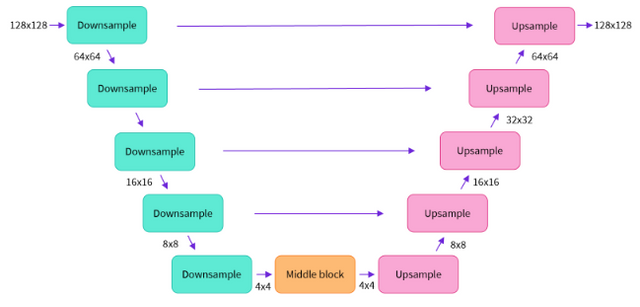
\includegraphics[width=0.8\linewidth]{images/dnn_example.png}
    \caption{Диффузионная нейронная сеть}
    \label{fig:dnn_example}
\end{figure}

Диффузионные модели демонстрируют высокое качество синтезированных изображений, зачастую превосходящие своих конкруентов в детализации и реалистичности. Помимо этого, процесс обучения является стабильным, поскольку происходят неизменяющиеся действия в рамках каждой отдельной генерации. К недостаткам модели можно отнести высокую требовательность к вычислительной машине, поскольку для каждой генерации требуется сделать большое количество операций итеративного очищения вектора от шума, что в теории может затруднить интеграцию модели для работы в реальном времени. Качество сгенерированных результатов сильно зависит от настройки планировщика шума. Таким образом, неправильно подобранные параметры планировщика шума могут сильно исказить результаты.

\subsubsection{Применение \texttt{DNN}}
Выбор именно \texttt{LaDI"=VITON} обоснован тем, что данное решение впервые предлагает подход через латентные диффузионные модели (\texttt{Latent Diffusion Models, LDM}). \texttt{LDM} включают в себя автокодировщик $\mathcal{A}$ с кодировщиком $\mathcal{E}$ и декодировщиком $\mathcal{D}$, модель \texttt{U"=Net}  деноизации текста с временными условиями $\epsilon_{\theta}$, а также кодировщик текста \texttt{CLIP} $T_E$, который принимает на вход $Y$. Обучение $\epsilon_{\theta}$ осуществляется через следующую функцию потерь:
\begin{gather}
    L = \mathbb{E}_{\mathcal{E}(I),Y, \epsilon \sim \mathcal{N}(0, 1), t}[||\epsilon - \epsilon_{\theta}(\phi, \psi)||_2^2],
\end{gather}
где $t$ представляет собой шаг диффузии, $\phi = z_t$, $z_t$ "--- закодированное изображение $\mathcal{E}(I)$, в котором был добавлен шум $\mathcal{N}(0, 1)$, и $\psi = [t, T_E(Y)]$.
Целью данного процесса является генерация нового изображения $\tilde{I}$ из исходного изображения $I$, сочетающее в себе $I$ и одежду, предоставленную пользователем. Общий вид модели можно увидеть на рисунке \ref{fig:ladi_pipeline} \cite{ladi}.
\begin{figure}[H]
    \centering
    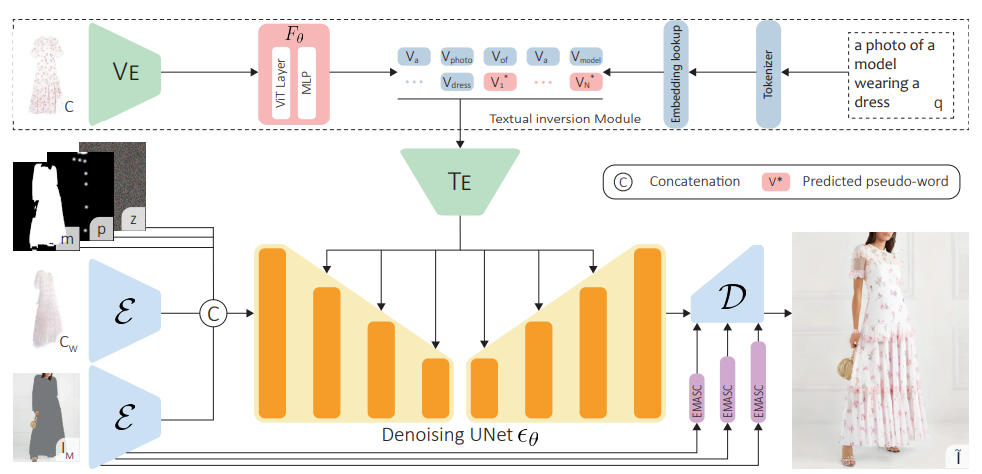
\includegraphics[width=0.94\linewidth]{images/ladi_pipeline.png}
    \caption{Общий вид \texttt{LADI"=VITON}}
    \label{fig:ladi_pipeline}
\end{figure}

Использование латентных диффузионных моделей позволяет работать в сжатом латентном пространстве, что снижает вычислительные затраты и повышает качество синтеза по сравнению с генерацией непосредственно в пиксельном пространстве. Текстовая инверсия с помощью \texttt{CLIP}-кодировщика эффективно кодирует визуальные характеристики одежды в условное пространство, обеспечивая точное управление процессом генерации и сохранение текстурных деталей. Модель \texttt{U-Net} с временными условиями обучается предсказывать шум на каждом шаге диффузии, что обеспечивает постепенное и стабильное восстановление изображения с учётом заданных условий. Дополнительные механизмы, такие как \texttt{Enhanced Mask-Aware Skip Connection} (\texttt{EMASC}), улучшают сохранение высокочастотных деталей и снижают ошибки реконструкции, что особенно важно для реалистичного отображения мелких деталей одежды. Обзор \texttt{EMASC} можно увидеть на рисунке \ref{fig:ladi_emasc} \cite{ladi}.
\begin{figure}[H]
    \centering
    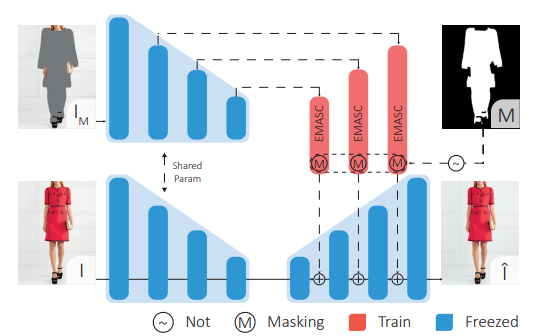
\includegraphics[width=0.9\linewidth]{images/ladi_emasc.png}
    \caption{Общий вид \texttt{EMASC}}
    \label{fig:ladi_emasc}
\end{figure}

Формально, модуль \texttt{EMASC} можно записать следующим образом:
\begin{gather}
    EMASC_i = f(E_i) * NOT(m_i) \\
    D_i = D_{i-1} + EMASC_i,
\end{gather}
где $f$ "--- обученная нелинейная функция, $E_i$ это $i$"=я карта признаков из кодировщика $\mathcal{E}$, $D_i$ есть соответствующая карта признаков из декодировщика, а $m_i$ получается в результате изменения размера маски $M$ в соответствии с пространственным измерением $E_i$.

Итоговая функция потерь имеет следующий вид:
\begin{gather}
    L = \mathbb{E}_{\mathcal{E}(I), \widehat{Y}, \epsilon \sim \mathcal{N}(0, 1),t,\mathcal{E}(I_M), M, p, \mathcal{E}(C_W)}[||\epsilon - \epsilon_{\theta}(\phi, \psi)||_2^2],
\end{gather}
где $\psi = [t;T_E(\widehat{Y})]$.